\section*{Part 3：Standardization 的影響}
\vspace{-0.5em}

\q{9}{無資料洩漏的標準化。}
\metric{StandardScaler} 只使用 455 筆訓練資料估計平均值與標準差，再以同一組參數轉換測試資料。資料切分及模型設定都維持不變，讓比較集中在標準化的影響。

\begin{minipage}{\linewidth}
\q{10}{四模型 Raw/Scaled 比較。}
\begin{center}
\compacttable
\begin{tabular}{lrrrrrr}
\toprule
分類器 & Raw Acc. & Scaled Acc. & $\Delta$Acc. & Raw F1 & Scaled F1 & $\Delta$F1 \\
\midrule
kNN & 0.9123 & 0.9561 & +0.0439 & 0.9066 & 0.9526 & +0.0460 \\
SVM & 0.9298 & 0.9825 & +0.0526 & 0.9230 & 0.9812 & +0.0582 \\
Decision Tree & 0.9123 & 0.9123 & 0.0000 & 0.9075 & 0.9075 & 0.0000 \\
Random Forest & 0.9561 & 0.9561 & 0.0000 & 0.9526 & 0.9526 & 0.0000 \\
\bottomrule
\end{tabular}
\end{center}
\end{minipage}

\q{11}{視覺比較。}
\begin{figure}[ht]
\centering
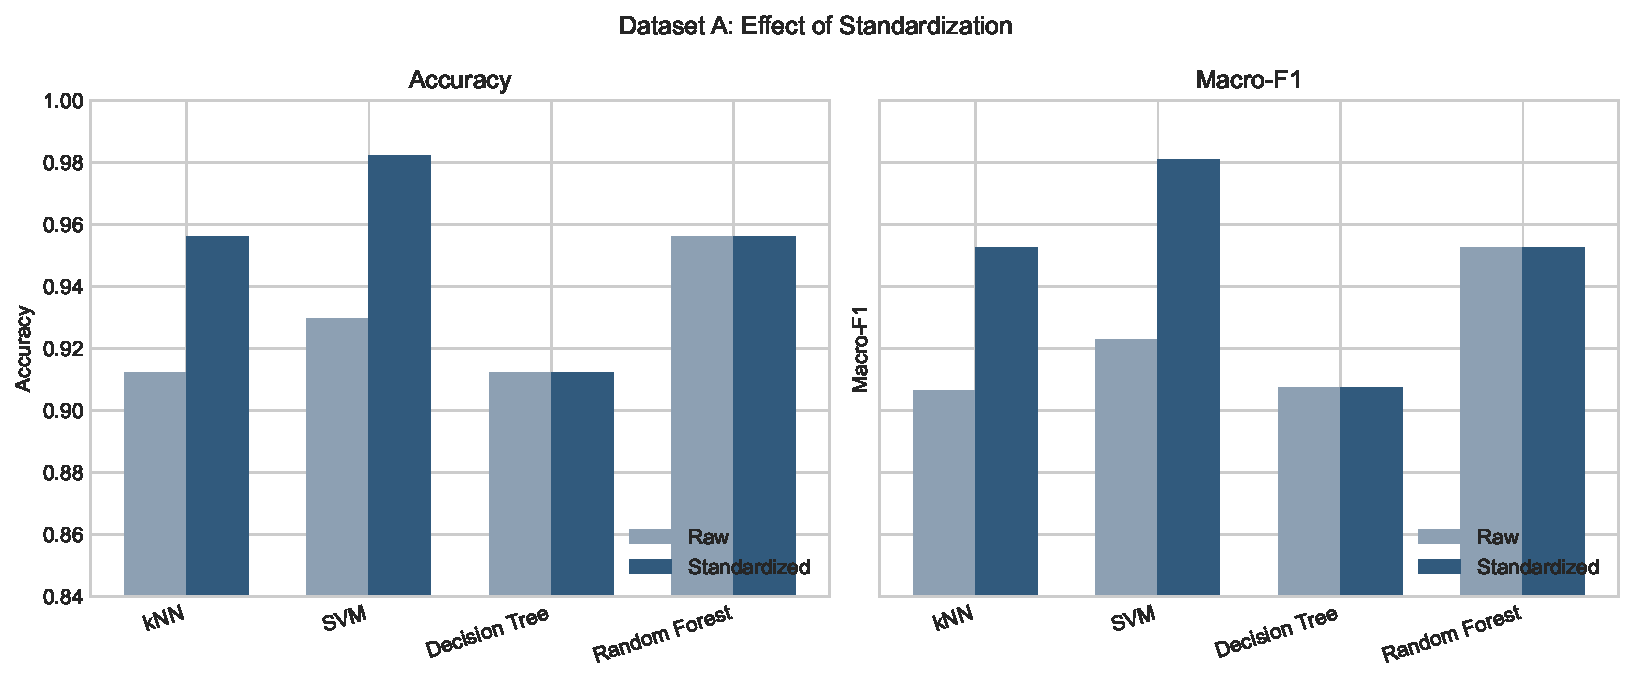
\includegraphics[width=0.78\linewidth]{standardization_comparison.pdf}
\caption{Dataset A 的 Raw/Scaled Accuracy 與 Macro-F1；圖值直接讀自 \metric{scaling\_a.csv}。}
\end{figure}

\q{12}{變化機制。}
SVM 的 Macro-F1 增加最多（+0.0582），其次是 kNN（+0.0460）。兩者都會受到特徵距離影響，若直接使用原始數值，area 等數值範圍大的特徵容易主導計算。標準化後，各特徵的影響較為均衡。相較之下，決策樹主要依單一特徵的大小順序決定分割點，因此這次 Decision Tree 與 Random Forest 的分數都沒有變化。

\q{13}{是否一定提升？}
不一定。這次 kNN 與 SVM 在標準化後都有明顯進步，但 Decision Tree 和 Random Forest 的 Accuracy、Macro-F1 都沒有改變。是否需要標準化，仍應依模型的運作方式與實際結果判斷。
